\de{ĐỀ THI HỌC KỲ I NĂM HỌC 2022-2023}{TRƯỜNG THPT Phùng Khắc Khoan - Hà Nội}

\begin{center}
	\textbf{PHẦN 1 - TRẮC NGHIỆM}
\end{center}
\Opensolutionfile{ans}[ans/ans]
\begin{ex}%[Dự án đề kiểm tra HKI NH22-23- Phan Hiếu]%[THPT PHÙNG KHẮC KHOAN -HN]%[0T5B3-3]%Câu 1%[0H2Y3-3]
    Trên đường thẳng $MN$ lấy điểm $P$ sao cho $\vec{MN}=-3\vec{MP}$. Điểm $P$ được xác định đúng trong hình vẽ nào sau đây?
    \begin{center}
        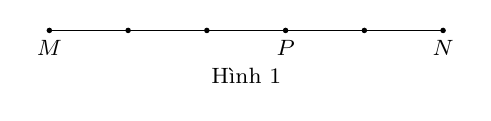
\begin{tikzpicture}[scale=1, font=\footnotesize, line join=round, line cap=round, >=stealth,x=1cm,y=1cm]
            \draw (0,0)node[below]{$M$}--(5,0)node[below]{$N$} (3,0)node[below]{$P$} (2.5,-.35)node[below]{Hình 1};
            \foreach \x in {0,1,2,3,4,5} {\fill (\x,0)circle(1pt);}
        \end{tikzpicture}
        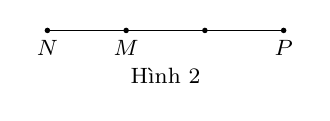
\begin{tikzpicture}[scale=1, font=\footnotesize, line join=round, line cap=round, >=stealth,x=1cm,y=1cm]
            \draw (0,0)node[below]{$N$}--(3,0)node[below]{$P$} (1,0)node[below]{$M$} (1.5,-.35)node[below]{Hình 2};
            \foreach \x in {0,1,2,3} {\fill (\x,0)circle(1pt);}
        \end{tikzpicture}\\[.5cm]
        
        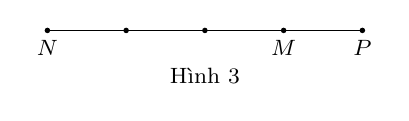
\begin{tikzpicture}[scale=1, font=\footnotesize, line join=round, line cap=round, >=stealth,x=1cm,y=1cm]
            \draw (0,0)node[below]{$N$}--(4,0)node[below]{$P$} (3,0)node[below]{$M$} (2,-.35)node[below]{Hình 3};
            \foreach \x in {0,1,2,3,4} {\fill (\x,0)circle(1pt);}
        \end{tikzpicture}
        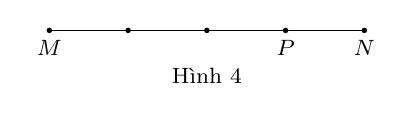
\begin{tikzpicture}[scale=1, font=\footnotesize, line join=round, line cap=round, >=stealth,x=1cm,y=1cm]
            \draw (0,0)node[below]{$M$}--(4,0)node[below]{$N$} (3,0)node[below]{$P$} (2,-.35)node[below]{Hình 4};
            \foreach \x in {0,1,2,3,4} {\fill (\x,0)circle(1pt);}
        \end{tikzpicture}
    \end{center}
    \choice
    {\True Hình $3$}
    {Hình $4$}
    {Hình $1$}
    {Hình $2$}
    \loigiai{
        Do $\vec{MN}=-3\vec{MP}$ nên $\vec{MN}$ ngược hướng với $\vec{MP}$ và $MN=3MP$.
    }
\end{ex}
\begin{ex}%[Dự án đề kiểm tra HKI NH22-23- Phan Hiếu]%[THPT PHÙNG KHẮC KHOAN -HN]%[0H2B4-1]
    Cho hình vuông $MNPQ$ có $I$, $J$ lần lượt là trung điểm của $PQ$, $M N$. Tích vô hướng của $\overrightarrow{QI} \cdot \overrightarrow{N J}$ bằng
    \choice
    {$\overrightarrow{P Q} \cdot \overrightarrow{P I}$}
    {$\overrightarrow{P Q} \cdot \overrightarrow{P N}$}
    {$\overrightarrow{P M} \cdot \overrightarrow{P Q}$}
    {\True $-\dfrac{\overrightarrow{P Q}^2}{4}$} 
    \loigiai
    {
        \immini
        {
            Ta có \begin{eqnarray*}
                \overrightarrow{QI} \cdot \overrightarrow{N J}&=&QI\cdot NJ\cdot \cos (\overrightarrow{QI}, \overrightarrow{N J})\\
                &=&QI\cdot NJ\cdot \cos 180^\circ=-\dfrac{\overrightarrow{P Q}^2}{4}.
            \end{eqnarray*} 
        }
        {
            \begin{tikzpicture}[>=stealth,line join=round,line cap=round,font=\footnotesize,scale=1]
                \def\a{3} %cạnh
                \path (0:0) coordinate (N)
                ++(0:\a) coordinate (P)
                ++(90:\a) coordinate (Q)
                ++(180:\a) coordinate (M);
                \draw (M)--(N)--(P)--(Q)--cycle;
                \coordinate (I) at ($(P)!0.5!(Q)$);
                \coordinate (J) at ($(M)!0.5!(N)$);
                \foreach \x/ \goc in {M/135,N/-135,P/-45,Q/45,J/180,I/0} 
                \fill (\x) circle (1pt)
                ($(\x)+(\goc:3mm)$) node {$\x$};
            \end{tikzpicture}
            
        }
    }
\end{ex}
\begin{ex}%[Dự án đề kiểm tra HKI NH22-23- Phan Hiếu]%[THPT PHÙNG KHẮC KHOAN -HN]%[0H2B2-5]
    Cho tam giác $ABC$ đều cạnh $a$, $H$ là trung điểm của $BC$. Giá trị của $|\overrightarrow{C A}-\overrightarrow{H C}|$ bằng
    \choice
    {$|\overrightarrow{C A}-\overrightarrow{H C}|=\dfrac{a}{2}$}
    {$|\overrightarrow{C A}-\overrightarrow{H C}|=\dfrac{3 a}{2}$}
    {$|\overrightarrow{C A}-\overrightarrow{H C}|=\dfrac{2 \sqrt{3} a}{3}$}
    {\True $|\overrightarrow{C A}-\overrightarrow{H C}|=\dfrac{a \sqrt{7}}{2}$} 
    \loigiai
    {
       \immini
       {
           Gọi $I$ là trung điểm $AH$.\\
           Ta có $AH=\dfrac{a\sqrt{3}}{2}$, $CI=\sqrt{HI^2+HC^2}=\sqrt{\dfrac{3a^2}{16}+\dfrac{a^2}{4}}=\dfrac{a \sqrt{7}}{4}$.\\
           Suy ra  $|\overrightarrow{C A}-\overrightarrow{H C}|=|\overrightarrow{C A}+\overrightarrow{CH}|=|2\overrightarrow{C I}|=2CI=\dfrac{a \sqrt{7}}{2}$.
       }
       {
          \begin{tikzpicture}[>=stealth,line join=round,line cap=round,line width=0.6pt,font=\footnotesize,scale=1]
              \coordinate[label=below left:$B$](B) at (0,0);
              \coordinate[label=below right:$C$](C) at (4,0);
              \coordinate[label=above left:$A$](A) at (2,3);
              \coordinate [label=below :$H$](H) at ($(B)!0.5!(C)$);
              \coordinate [label=right:$I$](I) at ($(H)!0.5!(A)$);
              \draw (A)--(B)--(C)--cycle;
              \draw[blue] (C)--(I) (A)--(H);
              \fill (A) circle (1.5pt) (B) circle (1.5pt) (C) circle (1.5pt) (H) circle (1.5pt) (I) circle (1.5pt);
         
          \end{tikzpicture}
           
       }
    }
\end{ex}
\begin{ex}%[Dự án đề kiểm tra HKI NH22-23- Phan Hiếu]%[THPT PHÙNG KHẮC KHOAN -HN]%[0H1Y1-3]
    Trong các đẳng thức sau, đẳng thức nào đúng?
    \choice
    {$\sin \left(180^{\circ}-\alpha\right)=-\cos \alpha$}
    {$\sin \left(180^{\circ}-\alpha\right)=-\sin \alpha$}
    {\True $\sin \left(180^{\circ}-\alpha\right)=\sin \alpha$}
    {$\sin \left(180^{\circ}-\alpha\right)=\cos \alpha$} 
    \loigiai
    {
        Ta có $\sin \left(180^{\circ}-\alpha\right)=\sin \alpha$.
    }
\end{ex}
\begin{ex}%[Dự án đề kiểm tra HKI NH22-23- Phan Hiếu]%[THPT PHÙNG KHẮC KHOAN -HN]%[0H1Y2-1]
    Cho tam giác $ABC$ tùy ý có $AB=c$, $AC=b$, $CB=a$. Mệnh đề nào dưới đây đúng?
    \choice
    {$c^2=a^2+b^2+2ab\cdot\cos C$}
    {\True $c^2=a^2+b^2-2ab\cdot\cos C$}
    {$c^2=a^2+b^2+ab\cdot\cos C$}
    {$c^2=a^2+b^2-ab\cdot\cos C$}
    \loigiai{
        Theo định lý Côsin trong tam giác $\triangle ABC$ ta có
        \begin{center}
            $c^2=a^2+b^2-2ab\cdot\cos C.$
        \end{center}	
    }
\end{ex}
\begin{ex}%[Dự án đề kiểm tra HKI NH22-23- Phan Hiếu]%[THPT PHÙNG KHẮC KHOAN -HN]%[0D1Y1-2]
    Trong các mệnh đề sau, mệnh đề nào là mệnh đề đúng?
    \choice
    {Tổng của hai số tự nhiên là một số chẵn khi và chỉ khi cả hai số đều là số chẵn}
    {Tích của hai số tự nhiên là một số chẵn khi và chỉ khi cả hai số đều là số chẵn}
    {Tổng của hai số tự nhiên là một số lẻ khi và chỉ khi cả hai số đều là số lẻ}
    {\True Tích của hai số tự nhiên là một số lẻ khi và chỉ khi cả hai số đều là số lẻ} 
    \loigiai
    {
        Tích của hai số tự nhiên là một số lẻ khi và chỉ khi cả hai số đều là số lẻ là mệnh đề đúng.
    }
\end{ex}
\begin{ex}%[Dự án đề kiểm tra HKI NH22-23- Phan Hiếu]%[THPT PHÙNG KHẮC KHOAN -HN]%[0H1B3-2]
    Khoảng cách từ $A$ đến $B$ không thể đo trực tiếp được vì phải qua một đầm lầy. Người ta xác định được một điểm $C$ mà từ đó có thể nhìn được $A$ và $B$ dưới một góc $78^{\circ} 24'$. Biết $C A=250 \mathrm{~m}, CB=120 \mathrm{~m}$. Khoảng cách $A B$ gần nhất với giá trị nào sau đây
    \choice
    {$266 \mathrm{~m}$}
    {\True $255 \mathrm{~m}$}
    {$166 \mathrm{~m}$}
    {$298 \mathrm{~m}$} 
    \loigiai
    {
        Ta có \begin{eqnarray*}
            AB^2&=&CA^2+CB^2-2\cdot CA\cdot CB\cdot \cos\widehat{ACB}\\
            &=&250^2+120^2-2\cdot 250\cdot 120\cdot \cos 78^\circ24'\simeq 254{,}63 ~\mathrm{m}.
        \end{eqnarray*}
    }
\end{ex}
\begin{ex}%[Dự án đề kiểm tra HKI NH22-23- Phan Hiếu]%[THPT PHÙNG KHẮC KHOAN -HN]%[0D1Y1-3]
    Cho mệnh đề \lq\lq$\forall x\in \mathbb{R},\, x^2-x+7<0$\rq\rq. Hỏi mệnh đề nào là mệnh đề phủ định của mệnh đề trên? 
    \choice
    {\True $\exists x\in \mathbb{R}, \, x^2-x+7\geq 0$}
    {$\forall x\in \mathbb{R},\, x^2-x+7>0$}
    {$\forall x\in \mathbb{R},\, x^2-x+7<0$}
    {$\nexists x\in \mathbb{R},\, x^2-x+7<0$}
    \loigiai{
        Mệnh đề phủ định của mệnh đề:~\lq\lq $\forall x\in \mathbb{R},\, x^2-x+7<0$\rq\rq ~là \lq\lq$\exists x\in \mathbb{R}, \, x^2-x+7\geq 0$\rq\rq.
    }
\end{ex}
\begin{ex}%[Dự án đề kiểm tra HKI NH22-23- Phan Hiếu]%[THPT PHÙNG KHẮC KHOAN -HN]%[0D4Y1-2]
    Cho tam thức bậc hai $f(x)=a x^2+b x+c \quad(a \neq 0)$. Điều kiện cần và đủ để\\ $f(x) \leq 0, \forall x \in \mathbb{R}$ là
    \choice
    {$\heva{&a<0  \\ &\Delta>0 }$}
    {$\heva{&a<0  \\ &\Delta>0 }$}
    {$\heva{& a>0 \\ & \Delta\ge 0}$}
    {\True $\heva{& a<0 \\ &\Delta\le 0 }$}
    \loigiai
    {
      Điều kiện cần và đủ để $f(x) \leq 0, \forall x \in \mathbb{R}$ là  $\heva{& a<0 \\ &\Delta\le 0. }$
    }
\end{ex}
\begin{ex}%[Dự án đề kiểm tra HKI NH22-23- Phan Hiếu]%[THPT PHÙNG KHẮC KHOAN -HN]%[0H1B2-3]
    Cho tam giác $A B C$ tùy ý có $B C=a, A C=b, A B=c$ và thoả mãn hệ thức $b+c=2 a$. Trong các mệnh đề sau, mệnh đề nào đúng ?
    \choice
    {$\cos B+\cos C=2 \cos A$}
    {\True $\sin B+\sin C=2 \sin A$}
    {$\sin B+\sin C=\dfrac{1}{2} \sin A$}
    {$\sin B+\cos C=2 \sin A$} 
    \loigiai
    {
      Ta có $b+c=2 a\Leftrightarrow \sin B\cdot 2R+ \sin C\cdot 2R=2\cdot \sin A\cdot 2R\Leftrightarrow \sin B+\sin C=2 \sin A$.  
    }
\end{ex}
\begin{ex}%[Dự án đề kiểm tra HKI NH22-23- Phan Hiếu]%[THPT PHÙNG KHẮC KHOAN -HN]%Câu 11%[0H2Y1-2]
    Cho tam giác $ABC$. Gọi $M$, $N$, $P$ lần lượt là trung điểm của $AB$, $BC$, $AC$. Các véc-tơ cùng phương với  $\vec{MN}$ là
    \choice
    {$\vec{AC},\vec{CA},\vec{AP},\vec{PA},\vec{PC},\vec{AM}$}
    {$\vec{NM},\vec{BC},\vec{CB},\vec{PA},\vec{AP}$}
    {\True $\vec{NM},\vec{AC},\vec{CA},\vec{AP},\vec{PA},\vec{PC},\vec{CP}$}
    {$\vec{NM},\vec{BC},\vec{CA},\vec{AM},\vec{MA},\vec{PN},\vec{CP}$}
    \loigiai{
        \immini{Ta có $MN$ là đường trung bình của tam giác $ABC$ nên $MN$  cùng phương với các véc-tơ $\vec{NM},\vec{AC},\vec{CA},\vec{AP},\vec{PA},\vec{PC},\vec{CP}$. }{\begin{tikzpicture}[line join = round, line cap = round,>=stealth,scale=0.7]
                \path
                (2,4) coordinate(A)
                (0,0) coordinate(B)
                (7,0) coordinate(C)
                ;
                \coordinate (M) at ($(A)! 0.5! (B)$);
                \coordinate (N) at ($(B)! 0.5! (C)$);
                \coordinate (P) at ($(A)! 0.5! (C)$);
                \draw (A)--(B)--(C)--cycle (M)--(N)--(P)--cycle;
                %\draw[dashed] (B)--(C) (M)--(N) (C)--(H);
                \foreach \d/\g in{A/90,B/-180,C/0,M/-180,N/-90,P/30}\draw[fill=black](\d)circle(1pt)+(\g:0.35)node{$\d$};
                \begin{scope}[on background layer]\path[white]node{MDD-129};\end{scope}
        \end{tikzpicture}}
    }
\end{ex}
\begin{ex}%[Dự án đề kiểm tra HKI NH22-23- Phan Hiếu]%[THPT PHÙNG KHẮC KHOAN -HN]%[0D2B2-2]
    \immini{Phần không gạch chéo ở hình sau đây biểu diễn miền nghiệm của hệ bất phương trình nào trong bốn hệ A, B, C, D?
        \choice
        {\True $\heva{&y >0\\& 3x+2y<6}$}
        {$\heva{&y >0\\& 3x+2y <-6}$}
        {$\heva{&x >0\\& 3x+2y<6}$}
        {$\heva{&x >0\\& 3x+2y>-6}$}}
    { \begin{tikzpicture}[scale=0.6, font=\footnotesize, line join=round, line cap=round, >=stealth]
            % \clip (-2.5,-1) rectangle (4,4.8);
            \draw[->] (-2,0)--(3.5,0) node[below]{$x$};
            \draw[->] (0,-2)--(0,4.5) node[left]{$y$};
            \fill[name=O] (0,0) circle (1pt) node[below left] {$O$}; 
            \draw[thick,blue] (-2/3,4)--(10/3,-2);
            \coordinate[label=below:{$2$}] (2x) at (2,0);
            \coordinate[label=left:{$3$}] (3y) at (0,3);
            \foreach \p in {2x,3y}
            \fill (\p) circle (1.2pt);
            \fill[pattern =north east lines,opacity=0.5,smooth] (-2/3,4)--(10/3,-2)--(3.5,-2)--(3.5,4)--cycle;
            \fill[pattern =north east lines,opacity=0.5,smooth] (-2,0)--(-2,-2)--(3,-2)--(3.5,0)--cycle;
    \end{tikzpicture}}
    \loigiai{
        Hai miền tô đen lần lượt có bờ là các đường thẳng $y=0$ và $3x+2y=6$.\\
        Ta có miền bị tô đen phía dưới trục hoành là phần mặt phẳng có $y<0$.\\
        Thay tọa độ $O(0,0)$ vào $3x+2y$ ta có $3\cdot 0 +2\cdot 0=0<6$.\\
        Suy ra nửa mặt phẳng bờ là đường thẳng $3x+2y=6$ chứa gốc tọa độ là miền biểu diễn cho bất phương trình $3x+2y<6$.\\
        Vậy miền tô đen trong hình là biểu diễn miền nghiệm của hệ $\heva{&y>0\\&3x+2y<6.}$
    }
\end{ex}
\begin{ex}%[Dự án đề kiểm tra HKI NH22-23- Phan Hiếu]%[THPT PHÙNG KHẮC KHOAN -HN]%[0H2Y1-4]
    Khẳng định nào sau đây đúng?
    \choice
    {Hai véc-tơ gọi là đối nhau nếu chúng có cùng độ dài}
    {\True Hai véc-tơ gọi là đối nhau nếu chúng ngược hướng và có cùng độ dài}
    {Hai véc-tơ gọi là đối nhau nếu chúng ngược hướng}
    {Hai véc-tơ gọi là đối nhau nếu chúng cùng phương và cùng độ dài}
    \loigiai
    {
        Hai véc-tơ gọi là đối nhau nếu chúng ngược hướng và có cùng độ dài là mệnh đề đúng.
    }
\end{ex}
\begin{ex}%[Dự án đề kiểm tra HKI NH22-23- Phan Hiếu]%[THPT PHÙNG KHẮC KHOAN -HN]%[0D1B2-2]
    Cho tập hợp $M=\{a ; b ; c ; d ; e\}$. Số tập con của tập $\mathrm{M}$ là
    \choice
    {\True $32$}
    {$25$}
    {$120$}
    {$5$} 
    \loigiai
    {
        Tập $M$ có $5$ phần tử nên có $2^5=32$ tập con.
    }
\end{ex}
\begin{ex}%[Dự án đề kiểm tra HKI NH22-23- Phan Hiếu]%[THPT PHÙNG KHẮC KHOAN -HN]%[0D4B3-2]
    Tập nghiệm $S$ của phương trình $\sqrt{2 x-3}=x-3$ là
    \choice
    {$S=\{6 ; 2\}$}
    {$S=\{2\}$}
    {\True $S=\{6\}$}
    {$S=\varnothing$} 
    \loigiai
    {
        Ta có $\sqrt{2 x-3}=x-3\Rightarrow 2x-3=(x-3)^2\Leftrightarrow x^2-8x+12=0\Leftrightarrow \hoac{&x=2  \\ &x=6. }$\\
        Thay lần lượt $x=2$ và $x=6$ vào phương trình ban đầu ta thấy $x=6$ là nghiệm.
    }
\end{ex}
\begin{ex}%[Dự án đề kiểm tra HKI NH22-23- Phan Hiếu]%[THPT PHÙNG KHẮC KHOAN -HN]%[0D1K3-4]
    Cho hai tập hợp $A=\left[-1;3\right)$ và $B=\left[a;a+3\right]$. Xác định giá trị của tham số $a$ sao cho $A\cap B=\varnothing$.
    \choice
    {\True $\hoac{&a\ge 3\\& a<-4}$}
    {$\hoac{&a>3\\&a\le-4}$}
    {$\hoac{&a\le 3\\&a\le -4}$}
    {$\hoac{&a<3\\&a\le-4}$}
    \loigiai{
        $A\cap B=\varnothing\Leftrightarrow\hoac{&a \ge 3\\&a+3<-1}\Leftrightarrow\hoac{&a\ge3\\&a<-4.}$
    }
\end{ex}
\begin{ex}%[Dự án đề kiểm tra HKI NH22-23- Phan Hiếu]%[THPT PHÙNG KHẮC KHOAN -HN]%[0D3K1-5]
    Xét sự biến thiên của hàm số $ y=\dfrac{1}{x^2}$. Mệnh đề nào sau đây \textbf{đúng}?
    \choice
    {\True Hàm số đồng biến trên $(-\infty ;0)$, nghịch biến trên $(0;+\infty)$}
    {Hàm số đồng biến trên $(0;+\infty)$, nghịch biến trên $(-\infty ;0)$}
    {Hàm số đồng biến trên $(-\infty ;1)$, nghịch biến trên $(1;+\infty)$}
    {Hàm số nghịch biến trên $(-\infty ;0)\cup(0;+\infty)$}
    \loigiai{
        TXĐ: $\mathscr{D}= \mathbb{R} \setminus \{0\}$. 
        \begin{itemize}
            \item Lấy $x_1, x_2 \in (0; +\infty): 0< x_1 < x_2$. Khi đó $x_2-x_1>0$ và $x_1+x_2>0$.\\
            Xét hiệu: $f(x_1) -f(x_2)= \dfrac{1}{x_1^2} - \dfrac{1}{x_2^2} = \dfrac{x_2^2-x_1^2}{x_1^2\cdot x_2^2}= \dfrac{(x_2-x_1)(x_2+x_1)}{x_1^2\cdot x_2^2} > 0$\\	$\Rightarrow f(x_1) > f(x_2)$.\\
            Suy ra hàm số nghịch biến trên khoảng $(0;+\infty)$.
            \item Lấy $x_1, x_2 \in (-\infty;0): x_1 < x_2<0$. Khi đó $x_2-x_1>0$ và $x_1+x_2<0$.\\
            Xét hiệu: $f(x_1)-f(x_2)= \dfrac{1}{x_1^2} - \dfrac{1}{x_2^2} = \dfrac{x_2^2-x_1^2}{x_1^2\cdot x_2^2}= \dfrac{(x_2-x_1)(x_2+x_1)}{x_1^2\cdot x_2^2} < 0$\\	$\Rightarrow f(x_1) < f(x_2)$.\\
            Suy ra hàm số đồng biến trên khoảng $(-\infty;0)$.
        \end{itemize}
        
        
    }
\end{ex}
\begin{ex}%[Dự án đề kiểm tra HKI NH22-23- Phan Hiếu]%[THPT PHÙNG KHẮC KHOAN -HN]%[0H2Y4-1]
    Tích vô hướng của hai véc-tơ $\vec{a}$ và $\vec{b}$ cùng khác $\overrightarrow{0}$ là số âm khi
    \choice
    {$\vec{a}$ và $\vec{b}$ cùng chiều}
    {$\vec{a}$ và $\vec{b}$ cùng phương}
    {$0<(\vec{a}, \vec{b})<90^{\circ}$}
    {\True $90^\circ<(\vec{a}, \vec{b})<180^{\circ}$} 
    \loigiai
    {
         Ta có $\vec{a}\cdot\vec{b}<0$ khi $90^\circ<(\vec{a}, \vec{b})<180^{\circ}$.
    }
\end{ex}
\begin{ex}%[Dự án đề kiểm tra HKI NH22-23- Phan Hiếu]%[THPT PHÙNG KHẮC KHOAN -HN]%[0H3B1-2]
    Cho tam giác $A B C$ với $A(-3 ; 6) ; B(9 ;-10)$ và $G\left(\dfrac{1}{3} ; 0\right)$ là trọng tâm. Tọa độ đỉnh $C$ là
    \choice
    { $C(5 ;-4)$}
    {$C(5 ; 4)$}
    {\True $C(-5 ; 4)$}
    {$C(-5 ;-4)$} 
    \loigiai
    {
        Ta có $\heva{& x_C=3x_G-x_A-x_B=1-(-3)-9=-5 \\ &  y_C=3y_G-y_A-y_B=0-6-(-10)=4}\Rightarrow C(-5 ; 4)$.
    }
\end{ex}
\begin{ex}%[Dự án đề kiểm tra HKI NH22-23- Phan Hiếu]%[THPT PHÙNG KHẮC KHOAN -HN]%[0D3B2-3]
    Nếu hàm số $y=ax^2+bx+c$ có $a<0$; $ b>0$ và $c>0$ thì đồ thị hàm số của nó là hình nào trong các hình sau?
    \choice
     {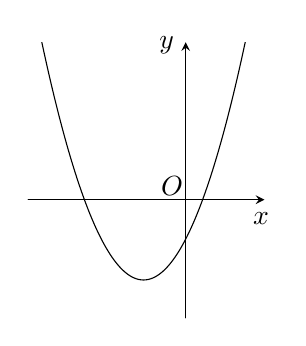
\begin{tikzpicture}[font=\footnotesize, line join=round, line cap=round, >=stealth]
            \tikzset{declare function={xmin=-2;xmax=1;ymin=-1.5;ymax=2;
                    f(\x)=1.81*(\x)^2+1.94*(\x)-0.5;
                },
                smooth,samples=450
            }
            \draw[->] (xmin,0)--(xmax,0) node[shift={(-100:7pt)},font=\normalsize]{$ x $};
            \draw[->] (0,ymin)--(0,ymax) node[shift={(190:7pt)},font=\normalsize]{$ y $};
            \fill (0,0) node[shift={(135:7pt)},font=\normalsize]{$ O $};
            \clip (xmin,ymin) rectangle (xmax,ymax);
            \draw  plot[domain=xmin:xmax] (\x, {f(\x)});
    \end{tikzpicture}}
  {\begin{tikzpicture}[font=\footnotesize, line join=round, line cap=round, >=stealth]
        \tikzset{declare function={xmin=-1;xmax=2;ymin=-1;ymax=3;
                f(\x)=1.99*(\x)^2-2.03*(\x)+1.19;
            },
            smooth,samples=450
        }
        \draw[->] (xmin,0)--(xmax,0) node[shift={(-100:7pt)},font=\normalsize]{$ x $};
        \draw[->] (0,ymin)--(0,ymax) node[shift={(190:7pt)},font=\normalsize]{$ y $};
        \fill (0,0) node[shift={(135:7pt)},font=\normalsize]{$ O $};
        \clip (xmin,ymin) rectangle (xmax,ymax);
        \draw  plot[domain=xmin:xmax] (\x, {f(\x)});
    \end{tikzpicture}}
    {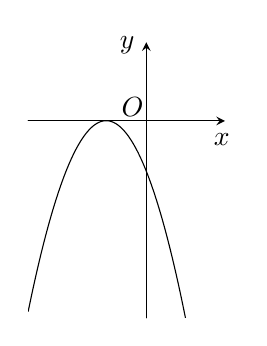
\begin{tikzpicture}[font=\footnotesize, line join=round, line cap=round, >=stealth]
            \tikzset{declare function={xmin=-1.5;xmax=1;ymin=-2.5;ymax=1;
                    f(\x)=-2.47*(\x)^2-2.52*(\x)-0.64;
                },
                smooth,samples=450
            }
            \draw[->] (xmin,0)--(xmax,0) node[shift={(-100:7pt)},font=\normalsize]{$ x $};
            \draw[->] (0,ymin)--(0,ymax) node[shift={(190:7pt)},font=\normalsize]{$ y $};
            \fill (0,0) node[shift={(135:7pt)},font=\normalsize]{$ O $};
            \clip (xmin,ymin) rectangle (xmax,ymax);
            \draw  plot[domain=xmin:xmax] (\x, {f(\x)});
    \end{tikzpicture}}
    {\True 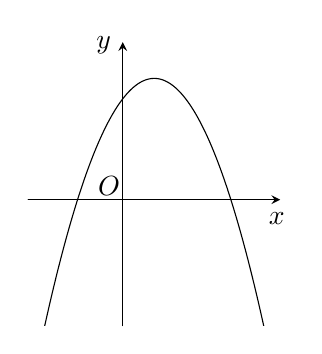
\begin{tikzpicture}[font=\footnotesize, line join=round, line cap=round, >=stealth,scale=0.8]
            \tikzset{declare function={xmin=-1.5;xmax=2.5;ymin=-2;ymax=2.5;
                    f(\x)=-1.3*(\x)^2+1.3*(\x)+1.6;
                },
                smooth,samples=450
            }
            \draw[->] (xmin,0)--(xmax,0) node[shift={(-100:7pt)},font=\normalsize]{$ x $};
            \draw[->] (0,ymin)--(0,ymax) node[shift={(190:7pt)},font=\normalsize]{$ y $};
            \fill (0,0) node[shift={(135:7pt)},font=\normalsize]{$ O $};
            \clip (xmin,ymin) rectangle (xmax,ymax);
            \draw  plot[domain=xmin:xmax] (\x, {f(\x)});
    \end{tikzpicture}}
    \loigiai{
        Đồ thị hàm số	$a<0$ nên bề lõm đồ thị quay xuống và $c>0$ nên đồ thị cắt trục $Oy$ phía trên $Ox $ nên ta chọn 
        \begin{center}
       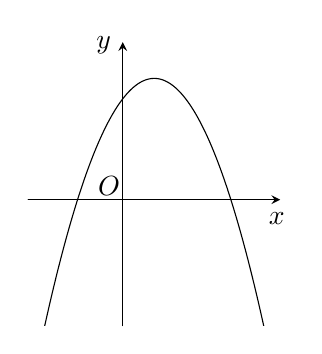
\begin{tikzpicture}[font=\footnotesize, line join=round, line cap=round, >=stealth,scale=0.8]
           \tikzset{declare function={xmin=-1.5;xmax=2.5;ymin=-2;ymax=2.5;
                   f(\x)=-1.3*(\x)^2+1.3*(\x)+1.6;
               },
               smooth,samples=450
           }
           \draw[->] (xmin,0)--(xmax,0) node[shift={(-100:7pt)},font=\normalsize]{$ x $};
           \draw[->] (0,ymin)--(0,ymax) node[shift={(190:7pt)},font=\normalsize]{$ y $};
           \fill (0,0) node[shift={(135:7pt)},font=\normalsize]{$ O $};
           \clip (xmin,ymin) rectangle (xmax,ymax);
           \draw  plot[domain=xmin:xmax] (\x, {f(\x)});
       \end{tikzpicture}
        \end{center}
    }
\end{ex}
\begin{ex}%[Dự án đề kiểm tra HKI NH22-23- Phan Hiếu]%[THPT PHÙNG KHẮC KHOAN -HN]%[0D4B2-1]
    Tam thức $y=x^2-12 x-13$ nhận giá trị âm khi và chỉ khi
    \choice
    {$x<-13$ hoặc $x>1$}
    {$x<-1$ hoặc $x>13$}
    {$-13<x<1$}
    {\True $-1<x<13$}
    \loigiai
    {
        Ta có $y=x^2-12 x-13<0 \Leftrightarrow -1<x<13$.
    }
\end{ex}
\begin{ex}%[Dự án đề kiểm tra HKI NH22-23- Phan Hiếu]%[THPT PHÙNG KHẮC KHOAN -HN]%[0H2B3-6]
    Cho tam giác đều $\mathrm{ABC}$ cạnh bằng $1$. Gọi $\mathrm{H}$ là trung điểm $\mathrm{BC}$. Giá trị của $|\overrightarrow{A H}|$ bằng
    \choice
    {\True $\dfrac{\sqrt{3}}{2}$}
    {$1$}
    {$2$}
    {$\sqrt{3}$} 
    \loigiai
    {
        Ta có $AH=\dfrac{AB\sqrt{3}}{2}=\dfrac{\sqrt{3}}{2}$.
    }
\end{ex}
\begin{ex}%[Dự án đề kiểm tra HKI NH22-23- Phan Hiếu]%[THPT PHÙNG KHẮC KHOAN -HN]%[0D3B2-1]
    Parabol $y=x^2-4 x+4$ có tọa độ đỉnh I là
    \choice
    {$I(1 ; 1)$}
    {\True $I(2 ; 0)$}
    {$I(-1 ; 1)$}
    {$I(-1 ; 2)$} 
    \loigiai
    {
        Ta có $a=1,b=-4$ nên tọa độ đỉnh $I(2;0)$.
    }
\end{ex}
\begin{ex}%[Dự án đề kiểm tra HKI NH22-23- Phan Hiếu]%[THPT PHÙNG KHẮC KHOAN -HN]%[0D2B1-2]
    Phần không bị gạch (không kể đường thẳng $d$) trong hình sau đây là miền nghiệm của bất phương trình nào?
    \begin{center}
        \begin{tikzpicture}[font=\footnotesize, line join = round, line cap = round, >=stealth, x=1cm, y=1cm, scale=.8]
            %---------------------- Vẽ hệ trục tọa độ
            \draw[->] (-4.5,0)--(3,0) node[below right] {$x$};
            \draw[->] (0,-2)--(0,4) node[right] {$y$};
            \node (0,0) [below left]{$ O $};
            \clip (-4.5,-2) rectangle (3,4);
            %----------------------- Vẽ đoạn chắn trên trục
            \foreach \x in {-4,-3,-2,-1,1,2,3}
            \draw[shift={(\x,0)},color=black] (0pt,2pt) -- (0pt,-2pt);
           \foreach \x in {-1,-2,-3,-4,1,2}\draw (\x,0) node[below]{$\x$} ;
            \foreach \y in {-1,1,2}\draw (0,\y) node[left]{$\y$} ;
            \foreach \y in {-1,1,2,3}
            \draw[shift={(0,\y)},color=black] (2pt,0pt) -- (-2pt,0pt);	
            %--------------------- Vẽ hàm
            \draw [thick, domain=-4.5:3, samples=100] plot (\x, {0.5*\x +2});
            %\node at (3.5,-2.75) {$(d)$};	
            %----------------------Vẽ miền nghiệm
            \fill[pattern=north east lines,opacity=.3] (-4.5,-0.2)--(-4.5,-2)--(3,-2)--(3,3.6)--cycle;			
        \end{tikzpicture}
    \end{center}
    \choice
    {$y+4>0$}
    {\True $x-2y+4<0$}
    {$x-y+4<0$}
    {$x-2y+4>0 $}
    \loigiai{
        Đường thẳng $\Delta $ đi qua $\left( -4;0 \right)$và $\left( 0;2 \right)$ có phương trình $x-2y+4=0$.\\
        Đặt $T\left( x;y \right)=x-2y+4$. \\
        Ta có $T\left( 0;0 \right)=4>0$
        nên gốc toạ độ $O$ không thuộc miền nghiệm của bất phương trình $x-2y+4<0$.
    }
\end{ex}
\begin{ex}%[Dự án đề kiểm tra HKI NH22-23- Phan Hiếu]%[THPT PHÙNG KHẮC KHOAN -HN]%[0D2B1-1]
    Miền nghiệm của hệ bất phương trình $\heva{& 3 x+y \geq 9  \\ & x \geq y-3\\&2 y \geq 8-x\\&3 x+y \geq 9}$ là phần mặt phẳng chứa điểm nào sau đây?
    \choice
    {$(0 ; 0)$}
    {$(1 ; 2)$}
    {$(2 ; 1)$}
    {\True $(8 ; 4)$} 
    \loigiai
    {
        Thay tọa độ $(8 ; 4)$ vào hệ bất phương trình đã cho ta thấy thỏa.\\
        Vậy miền nghiệm của hệ chứa điểm $(8 ; 4)$.
    }
\end{ex}
\Closesolutionfile{ans}
%\begin{center}
%	\textbf{ĐÁP ÁN}
%	\inputansbox{10}{ans/ans}	
%\end{center}

\begin{center}
	\textbf{PHẦN 2 - TỰ LUẬN}
\end{center}


\begin{bt}%[0D1B3-4]%[Dự án đề kiểm tra HK1 22-23-Nhật Thiện]%[Trường THPT PHÙNG KHẮC KHOAN, HÀ NỘI]
	Cho các tập hợp $M=[-3;6]$ và $N=(-\infty;-2)\cup  (3;+\infty)$. Tìm  tập $M\cap N$ và biểu diễn tập đó trên trục số.
	\loigiai{
	Ta có $M=[-3;6]$ và $N=(-\infty;-2)\cup (3;+\infty)$.\\
	Khi đó $M\cap N=[-3;-2)\cup (3;6]$.\\
	Biểu diễn trên trục số
	\begin{center}
		\begin{tikzpicture}[scale=1, font=\footnotesize, line join=round, line cap=round, >=stealth]
			\fill[pattern=north east lines](-4,-0.15)rectangle(-3,0.15);
			\draw[->] (-4,0)--(7,0);
			\draw (-3,0) node {$\big[$} (-3,0) node[below=6pt]{$-3$};
			\draw (-2,0) node {$\big)$} (-2,0) node[below=6pt]{$-2$};
			\fill[pattern=north east lines](-2,-0.15)rectangle(3,0.15);
			\draw (3,0) node {$\big($} (3,0) node[below=6pt]{$3$};
			\draw (6,0) node {$\big]$} (6,0) node[below=6pt]{$6$};
			\fill[pattern=north east lines](6,-0.15)rectangle(7,0.15);
		\end{tikzpicture}
	\end{center}
}
\end{bt}
\begin{bt}%[0H1K3-2]%[Dự án đề kiểm tra HK1 22-23-Nhật Thiện]%[Trường THPT PHÙNG KHẮC KHOAN, HÀ NỘI]
	\immini{Muốn đo chiều cao của tháp chàm Por Klong Garai ở Ninh Thuận người ta lấy hai điểm $A$ và $B$ trên mặt đất có khoảng cách $AB=12$ m cùng thẳng hàng với chân $C$ của tháp để đặt hai giác kế. Chân của giác kế có chiều cao $h=1{,}3$ m. Gọi $D$ là đỉnh tháp và hai điểm $A_1$, $B_1$ cùng thẳng hàng với $C_1$ thuộc chiều cao $CD$ của tháp. Người ta đo được góc $\widehat{DA_1C_1}=49^\circ$ và $\widehat{DB_1C_1}=35^\circ$. Tính chiều cao $CD$ của tháp.}{
	\begin{tikzpicture}[scale=1, font=\footnotesize, line join=round, line cap=round, >=stealth]
		\path 
		(0,0) coordinate (C)
		(0,4) coordinate (D)
		(3,0) coordinate (A)
		(5,0) coordinate (B)
		(0,1) coordinate (C_1)
		(3,1) coordinate (A_1)
		(5,1) coordinate (B_1)
		;
		\draw (B)--(C)--(D) (C_1)--(B_1) (A)--(A_1)--(D) (B)--(B_1)--(D);
		\path 
		(C)--node[midway,right]{$1{,}3$ m} (C_1)
		(A)--node[midway,below]{$12$ m} (B)
		(A_1)--node[midway,below]{$12$ m} (B_1)
		;
		\foreach \x/\dinh/\y in {D/C_1/B_1} \draw[fill = gray!50] ($(\dinh)!5pt!(\x)$)--($(\dinh)!5pt!(\x)+(\dinh)!5pt!(\y)-(\dinh)$)--($(\dinh)!5pt!(\y)$)--(\dinh)--cycle; 
		\foreach \p/\r in {A/-90,B/-90,C/-90,C_1/180,D/150,A_1/45,B_1/45}
		\fill (\p) circle (1.5pt) node[shift={(\r:3mm)}]{$\p$};
		\draw    pic["$49^\circ$", draw=black, angle eccentricity=1.2, angle radius=0.8cm]
		{angle=D--A_1--C_1}; %góc
		\draw    pic["$35^\circ$", draw=black, angle eccentricity=1.2, angle radius=0.8cm]
		{angle=D--B_1--C_1}; %góc
	\end{tikzpicture}
}
	\loigiai{
	Ta có $\widehat{C_1DA_1}=90^\circ-49^\circ=\widehat{41}$; $\widehat{C_1DB_1}=90^\circ-35^\circ=55^\circ$, nên $\widehat{A_1DB_1}=14^\circ$.\\
	Xét tam giác $A_1DB_1$, có 
	$$\dfrac{A_1B_1}{\sin \widehat{A_1DB_1}}=\dfrac{A_1D}{\sin \widehat{A_1B_1D}}\Rightarrow A_1D=\dfrac{12\cdot \sin 35^\circ}{\sin 14^\circ}\approx 28{,}45\text{ m}.$$
	Xét tam giác $C_1A_1D$ vuông tại $C_1$, có
	$$\sin \widehat{C_1A_1D}=\dfrac{C_1D}{A_1D}\Rightarrow C_1D=A_1D\cdot \sin \widehat{C_1A_1D}=28{,}45\cdot \sin 49^\circ\approx 21{,}47\text{ m}.$$
	Suy ra $CD=C_1D+CC_1\approx 22{,}77$ m.\\
	Vậy chiều cao $CD$ của tháp là $22{,}77$ m.
}
\end{bt}
\begin{bt}%[0D3K2-5]%[Dự án đề kiểm tra HK1 22-23-Nhật Thiện]%[Trường THPT PHÙNG KHẮC KHOAN, HÀ NỘI]
	\immini{Cổng Arch tại thành phố St Louis của Mỹ có hình dạng là một parabol (hình vẽ). Biết khoảng cách giữa hai chân cổng bằng $162$ m. Trên thành cổng, tại vị trí có độ cao $43$ m so với mặt đất (điểm $M$), người ta thả một sợi dây chạm đất (dây căng thẳng theo phương vuông góc với mặt đất). Vị trí chạm đất của đầu sợi dây này cách chân cổng $A$ một đoạn $10$ m. Giả sử các số liệu trên là chính xác. Hãy tính độ cao của cổng Arch (tính từ mặt đất đến điểm cao nhất của cổng).}{
	\begin{tikzpicture}[>=stealth,line join=round,line cap=round, font=\footnotesize,scale=.8]
		\def\f(\x){-0.56*(\x)^2+3.33*(\x)}
		\path
		(0,0)coordinate (A)node[below left]{$A$}
		(6,0)coordinate (B)node[below]{$B$}
		(1,2.78)coordinate (M)node[below right]{$M$}
		(1,0)coordinate (C)
		;
		\draw[smooth,blue] plot[domain=0:6](\x,{\f(\x)});
		\draw[dashed] (A)--(B)node[midway,above]{$162$ m} (C)--(M)node[midway,right]{$43$ m};
		\draw[<->](A)--(C)node[midway,below]{$10$ m};
		\foreach \x in{A,B,M} \fill[black] (\x)circle (1.5pt);
	\end{tikzpicture}
}
	\loigiai{
	\immini{Chọn hệ trục tọa độ $Oxy$ như hình vẽ. Phương trình Parabol $(P)$ có dạng $y=ax^2+bx+c$. \\
	Phương trình $(P)$ đi qua điểm $A(0;0)$, $B(162;0)$ và $M(10;43)$ nên ta có
	$$\heva{&c=0\\&162^2 a+162 b+c=0\\&10^a+10b+c=43}\Leftrightarrow \heva{&c=0\\&a=-\dfrac{43}{1520}\\&b=\dfrac{3483}{760}.}$$
	Suy ra $(P)\colon y=-\dfrac{43}{1520}x^2+\dfrac{3483}{760}x$.}{\begin{tikzpicture}[>=stealth,line join=round,line cap=round, font=\footnotesize,scale=.8]
		\def\f(\x){-0.56*(\x)^2+10/3*(\x)}
		\path
		(0,0)coordinate (A)node[below left]{$A$}
		(6,0)coordinate (B)node[below]{$B$}
		(1,2.78)coordinate (M)node[below right]{$M$}
		(1,0)coordinate (C)
		;
		\draw[smooth,blue] plot[domain=0:5.95](\x,{\f(\x)});
		\draw[dashed] (A)--(B)node[midway,above]{$162$ m} (C)--(M)node[midway,right]{$43$ m};
		\draw[<->](A)--(C)node[midway,below]{$10$ m};
		\draw[->](-1,0)--(7,0)node[below]{$x$};
		\draw[->](0,-1)--(0,5.5)node[left]{$y$};
		\foreach \x in{A,B,M} \fill[black] (\x)circle (1.5pt);
	\end{tikzpicture}
}
	\noindent Do đó chiều cao của cổng là $h=-\dfrac{\Delta}{4a}=-\dfrac{b^2-4ac}{4a}\approx 185{,}6$ (m).\\
	Vậy chiều cao của cổng $h\approx 185{,}6$ (m).
}
\end{bt}
\begin{bt}%[0D3K2-4]%[Dự án đề kiểm tra HK1 22-23-Nhật Thiện]%[Trường THPT PHÙNG KHẮC KHOAN, HÀ NỘI]
	Tìm tất các các giá trị của tham số $m$ để đường thẳng $d\colon y=2x+3$ cắt parabol $y=x^2+(m+2)x-m$ tại hai điểm phân biệt nằm cùng phía với trục tung $Oy$.
	\loigiai{
	Xét phương trình hoành độ giao điểm
	$$x^2+(m+2)x-m=2x+3\Leftrightarrow x^2+mx-m-3=0.\qquad(1)$$
	Để đường thẳng $d$ cắt parabol tại hai điểm phân biệt nằm cùng phía với trục tung $Oy$ thì phương trình $(1)$ có hai nghiệm phân biệt cùng dấu 
	$$\Leftrightarrow \heva{&\Delta>0\\&\dfrac{c}{a}>0}\Leftrightarrow \heva{&m^2+4m+12>0\\&-m-3>0}\Leftrightarrow m<-3.$$
	Vậy $m<-3$ thỏa mãn yêu cầu bài toán.
}
\end{bt}
\begin{bt}%[0H2B3-5]%[Dự án đề kiểm tra HK1 22-23-Nhật Thiện]%[Trường THPT PHÙNG KHẮC KHOAN, HÀ NỘI]
	Cho tam giác $ABC$. Gọi $I$, $J$ là hai điểm xác định bởi các đẳng thức $\vec{IA}=2\vec{IB}$, $3\vec{JA}+2\vec{JC}=\vec{0}$. Hãy phân tích $\vec{IJ}$ theo $\vec{AB}$ và $\vec{AC}$.
	\loigiai{
	Ta có $\vec{IJ}=\vec{IA}+\vec{AJ}$.\\
	Mặt khác $\vec{IA}=-2\vec{AB}$ và $\vec{AJ}=\dfrac{2}{5}\vec{AC}$.\\
	Suy ra $\vec{IJ}=\dfrac{2}{5}\vec{AC}-2\vec{AB}$.\\
	Vậy $\vec{IJ}=\dfrac{2}{5}\vec{AC}-2\vec{AB}$.
}
\end{bt}